\section*{Weird and Wonderful Stories}

\subsection*{Bell's Bar Bet}
A classical statistician and a quantum physicist walk into a bar\footnote{%
  ``You'd have thought the second one would have noticed.'' --- Steven
  Wright%
}. They play a game recording only joint observations between systems, then
calculating a particular sum of the values. Both are well versed in
classical probability theory, their observations are flawless, and they
play fair. They take turns choosing systems from around the tavern and the
calculation always yields $2$ or less, which comes as no surprise to either
of them. 

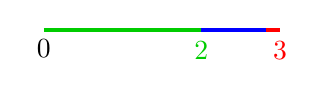
\begin{tikzpicture}
  \node [below] (0, 0) {$0$};
  \draw [ultra thick, green!80!black] (0,0) -- (2,0) node [below] {$2$};
  \draw [ultra thick, blue] (2,0) -- (2.828, 0);
  \draw [ultra thick, red] (2.828, 0) -- (3, 0) node [below] {$3$};
\end{tikzpicture}

Now comes the hustle. The physicist pulls two \emph{entangled
  systems} from her pocket and bets the other a drink that this round of the
game will yield a value greater than $2$. The statistician salivates for
the Seagram's coming from this sucker bet. They play the game and obtain
the value $2.5$. The physicist figures something must have jumbled in her
pocket because she expected about $2.8$. She shrugs and orders a tea;
physicists like tea.

\subsection*{Better Tales}
\begin{footnotesize}
  
\begin{itemize}
\item \textsf{In Search of Schr\"odinger's Cat} by John Gribbin
\item \textsf{Feynman Lectures on Computation} by Richard P. Feynman
  (edited by Tony Hey and Robin W. Allen)
\item \textsf{The Quantum World} by J.C. Polkinghorne
\item \textsf{Mr. Tompkins in Paperback} by George Gamow
\item \textsf{Alice in Quantumland} by Robert Gilmore
\item \textsf{Quantum Computing Since Democritus} by Scott Aaronson
\end{itemize}
\end{footnotesize}